% Chapter 3: Scope of the project

\chapter{\company\ Heatmap }

\label{chapter03}

%-----------------
%   SECTION 3.1
%-----------------

\section{Definition of the problem} \label{problem}

%In any moment, \company\ uses user sessions or user queries to guess trends.
In any team of \company, the user queries and the providers data is compared in order to guess valuable trends for different \nameref{stakeholders}.
\\\\
Found that gap, a bunch of new ideas appeared. After some talks with product owners of different squads and some senior engineers a promising idea showed up:
\\\\
Comparison of \textbf{user demand} and \textbf{flights offered} by airlines, enabling finding \textit{over-requested} routes or airports. 
\\\\
\squad manages a huge amount of data: All flights planned for the next two years, this are more than 75 million records. The database of all user queries in the website or mobile application is even bigger\footnote{For instance, if there were only one query per visitor the database would have 4 million new records per day}. Not much more information needed to say that this is \textbf{Big Data} problem.
\\\\
With \squad's product owner help, we found some use cases for the professing of those 75 million routes and all user session's queries to get some significant results.
\\\\
Provide a visual tool to find routes and airports with much more demand than offer and be able to observe the evolution of it through time:

\begin{itemize}
  \item A route or airport with a lot of demand but not enough offer to cover it will be \textbf{over-requested}.
  \item A route or airport with much more offer but not that amount of demand will be \textbf{non-profitable}.
\end{itemize}

%-----------------
%   SECTION 3.2
%-----------------

\section{Scope}

Merging both data sources (providers and users) generates a lot of new valuable data with a lot of different application: From simply selling it to stakeholders, to complex deep learning systems.
\\\\
The final goal of this project is displaying the comparison in a simple Web UI for Marketing Squads or Tribes. This can be split in three smaller goals or components:

\subsection{Pipeline}

Distributed application that maps and merge all the data from both sources in its given format, to the required data model.
\\\\
The pipeline reads from \nameref{mp_engine} and \nameref{data_tribe} services. Then, the pipeline, maps the provider and user data to the desired data model. The new entities are stored in a database where the service will read from.
\\\\
The application will be split in two sub applications, one for providers' data and other for users'. So both can vary independently without depending on the each others' sources and changes may have in the future.

\subsection{Service}

Simple HTTP Service with a basic Application Programming Interface to \textbf{get} Pipeline's results. The service will have an internal endpoint only available for other \company\ applications or developers.

\subsection{Visual representation} \label{visual_representation}

Website with a visual representation of the data. There are plenty of ways to draw charts and maps visualizations.
\\\\
The Web UI will be composed by three main pages:

\subsubsection*{World Map}

Interactive world map with all airports represented with a dot. The radius of the dot depends on the amount of flights it operates.
\\\\
The user will be able to select an airport set a date and go to \nameref{chart_visualization} page. Another option is to select two airports, first the origin, then the destination, set a date and go to the \nameref{chart_visualization} page. If the user does not want to select the entity through the map, he/she can search it using the \nameref{browser}

\begin{figure}[H]
\centering
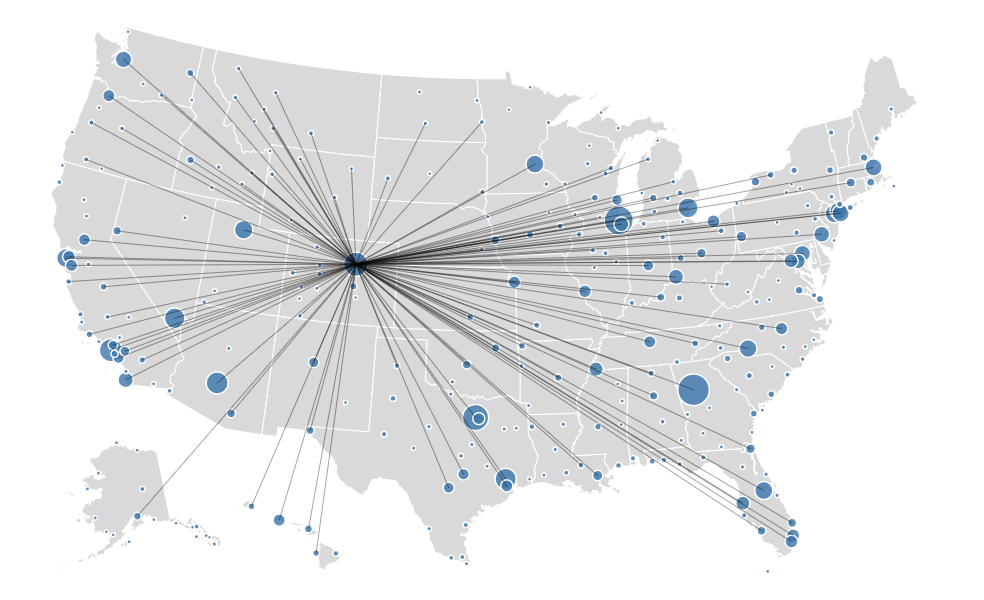
\includegraphics[scale=0.25]{resources/us-map-example01.png}
\caption{Example of how the world map style. Only displaying the US make it look clearer.}
\end{figure}

\subsubsection*{Browser} \label{browser}

Simple browser with two tabs: \textit{Route} and \textit{Airport}. In the route browser will appear three input text fields, one for the origin airport, the second for the destination and the last one for the date. In the airport browser will only appear two input text fields, airport and date.
\\\\
Once the inputs are set, the user will be able to click a \textit{Search} button and move to the next page, \nameref{chart_visualization}.

\subsubsection*{Chart visualization} \label{chart_visualization}

Simple chart with the comparison between providers offer and user demand of the selected entity through time.

\begin{figure}[H]
\centering
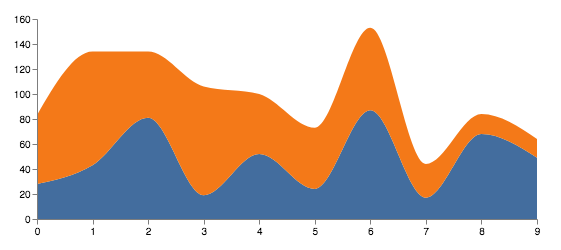
\includegraphics[scale=0.4]{resources/stacked-chart-example01.png}
\caption{Chart mock-up. One color goes for Providers Offer and the other one for User Demand.}
\end{figure}

\subsection{Not list}

It is also important to define what this project will \textbf{not} be.

% WIP
\begin{itemize}
  \item \textbf{Prices} or \textbf{quotes}: In any moment will check for flight prices or quotes.
  \item \textbf{Carriers}, \textbf{cities} and \textbf{countries}: The comparison will be only available between routes and airports, not airlines (carriers), cities nor countries.
  \item \textbf{Create}, \textbf{update} or \textbf{delete} data through the \textbf{Server}: The only input will come from the pipeline. Entities are never deleted or modified in order to keep historical data.
  \item \textbf{Create}, \textbf{update} or \textbf{delete} data through the \textbf{Web UI}: The only input will come from the pipeline. Entities are never deleted or modified in order to keep historical data.
\end{itemize}

%-----------------
%   SECTION 3.3
%-----------------

\section{Risks}

There are several risks can appear while developing the project. Most risks appear because of the dependencies with other tribes and squads, dependencies with other services. In the other hand, all performance risks of the Pipeline can ignored because \company's hardware is enough for big applications like this one.

\subsection{Routes contract}

\squad's routes service is under development and during the Heatmap development the routes' data model may change a little bit. For example, the origin and destination recently changed, in December 2017 their service was giving an \textit{Airport ID}, but now are given in an Airport object with more parameters like IATA Code\cite{iata_code}, Country ID, City ID, etc.

\subsection{Users information}

In the website and mobile application, the user have plenty of different ways to search the perfect flight. The most common one is by origin, destination and date, but he/she can also search by month, by destination. This way the user search flights may be difficult to compare with routes and airports offer because, sometimes, the route is the actual result.
\\\\
The user does not search flights for a given route in a given date. It sets the period of time he/she can travel and \company\ offers cheap destinations.

\subsection{Amount of data}

As explained before in the \nameref{problem}, there is a very big amount of data that need to be mapped. Luckily, \company\ have great cloud machines and (almost) unlimited space. But stills an issue to be aware of.

\subsection{Web UI}

Creating the interactive map and graphics of the proposed website from zero is a whole project itself. In order to avoid failing to the \nameref{visual_representation} goal, the best option is to use reliable libraries, like Vega\cite{vega}.

%-----------------
%   SECTION 3.4
%-----------------

\section{Methodology and rigor}

\subsection{Extreme Programming}

This project will be developed along with \squad's work. This squad is following Scrum, an agile methodology. After come research and some discussions with the rest of the team, Extreme Programming\cite{xp} showed up as the best option.
\\\\
XP is a style of software development focused in excellent applications, programming techniques, clear communication, etc. To accomplish that, XP includes a philosophy of software development, body of practices, complementary principles and a community that shares these values.
\\\\
This methodology works with short development cycles, resulting in early, concrete and continuing feedback. Has an incremental approach, making way to a flexible schedule of the implementation. It relies in oral communication and tests to reach the goal of the project.
\\\\
The original Extreme Programming methodology is for teams of developers, but this project will be only developed by myself, so the original idea has been modified a little bit. The pair programming and pair negotiation has been removed because I have nobody to pair with.

\begin{figure}[H]
\centering

\includegraphics[scale=0.2]{diagrams/extreme_programming.png}
\caption{Extreme programming planning loops.}
\end{figure}

\subsection{GitLab}

This platform will be the main tool for version control of the source code and issue tracking of different tasks.

\subsubsection*{\texttt{git}}

All code projects (pipelines, service and website) will be stored in my personal projects space in \company's GitLab domain. Tasks and issue projects will be related to each project.
\\\\
Using \texttt{git}, the versions will be forked in branches, each branch will stand for an specific issue. \textit{Master} will be the main branch where the latest production version will be.

\subsubsection*{Tasks and issues}

The \textbf{issue tracking} will be very helpful in order to monitor the evolution of the project. Issues will be composed by a title, description, milestone, labels (if needed), due date and weight, and represents a new functionality. In order to know the status, issues will be listed in three columns:

\paragraph*{Backlog:}

Known tasks that haven been started yet. Could be a well defined task, with a very clear description, due date and weight, or just a draft.

\paragraph*{WIP:}

Work in Progress. The task is being considered, developed or tested.

\paragraph*{Done:}

Tasks finished, tested and done. Ready for production.
